\documentclass[12px]{article}

\title{Lezione 26 Geometria I}
\date{2024-05-09}
\author{Federico De Sisti}

\usepackage{amsmath}
\usepackage{amsthm}
\usepackage{mdframed}
\usepackage{amssymb}
\usepackage{nicematrix}
\usepackage{amsfonts}
\usepackage{tcolorbox}
\tcbuselibrary{theorems}
\usepackage{xcolor}
\usepackage{cancel}

\newtheoremstyle{break}
  {1px}{1px}%
  {\itshape}{}%
  {\bfseries}{}%
  {\newline}{}%
\theoremstyle{break}
\newtheorem{theo}{Teorema}
\theoremstyle{break}
\newtheorem{lemma}{Lemma}
\theoremstyle{break}
\newtheorem{defin}{Definizione}
\theoremstyle{break}
\newtheorem{propo}{Proposizione}
\theoremstyle{break}
\newtheorem*{dimo}{Dimostrazione}
\theoremstyle{break}
\newtheorem*{es}{Esempio}

\newenvironment{dimo}
  {\begin{dimostrazione}}
  {\hfill\square\end{dimostrazione}}

\newenvironment{teo}
{\begin{mdframed}[linecolor=red, backgroundcolor=red!10]\begin{theo}}
  {\end{theo}\end{mdframed}}

\newenvironment{nome}
{\begin{mdframed}[linecolor=green, backgroundcolor=green!10]\begin{nomen}}
  {\end{nomen}\end{mdframed}}

\newenvironment{prop}
{\begin{mdframed}[linecolor=red, backgroundcolor=red!10]\begin{propo}}
  {\end{propo}\end{mdframed}}

\newenvironment{defi}
{\begin{mdframed}[linecolor=orange, backgroundcolor=orange!10]\begin{defin}}
  {\end{defin}\end{mdframed}}

\newenvironment{lemm}
{\begin{mdframed}[linecolor=red, backgroundcolor=red!10]\begin{lemma}}
  {\end{lemma}\end{mdframed}}

\newcommand{\icol}[1]{% inline column vector
  \left(\begin{smallmatrix}#1\end{smallmatrix}\right)%
}

\newcommand{\irow}[1]{% inline row vector
  \begin{smallmatrix}(#1)\end{smallmatrix}%
}

\newcommand{\matrice}[1]{% inline column vector
  \begin{pmatrix}#1\end{pmatrix}%
}

\newcommand{\C}{\mathbb{C}}
\newcommand{\K}{\mathbb{K}}
\newcommand{\R}{\mathbb{R}}


\begin{document}
	\maketitle
	\newpage
	\section{Mappe tra spazi proiettivi}
		Siano $V,W$ $\K$-spazi vettoriali
	\begin{defi}
		Un'applicazione $f:\pro(V) \rightarrow\pro(W)$ si dice trasformazione proiettiva se esiste un'applicazione lineare iniettiva $\varphi : V \rightarrow W$ tale che 
		\[
			f([v])=[ \varphi(v)] \ \ \ \forall \ v  \in V\setminus\{0\}
		.\] 
	\end{defi}
	\textbf{Osservazione}\\
	Scriviamo $f = \bar{\varphi}$ e diciamo che $\varphi$ induce $f$.\\
	Notiamo che $\bar{\varphi} = \overline{ \lambda \varphi} \ \ \ \ \lambda\in \R\setminus\{0\}$ quindi la famiglia $\{ \lambda \varphi | \lambda\in \K\setminus\{0\}$ induce la stessa trasformazione proiettiva
	\begin{nome}
		$\circ$ Se $\varphi$ è un isomorfismo $f=\bar \varphi$ si chiama isomorfismo proiettivo\\
		$\circ$ Se $\varphi : V \rightarrow V$ è un isomorfismo, $f=\bar \varphi$ si chiama proiettività\\
		$\circ$ $A,B\subseteq\pro(V)$ sono proiettivamente equivalenti se esiste proettività $f$ tale che $f(A)=B$
	\end{nome}
	\textbf{Formula di Grassmann Proiettiva}\\
	$S_1 = \pro(W_1) \ \ S_2 = \pro(W_2)$\\
	$S_1\cap S_2=\pro(W_1\cap W_2)$ $\ \ \ L(S_1,S_2) = \pro(W_1+W_2)$\\
	Dove $L(S_1,S_2)$ è il minimo sottospazio che contiene $S_1,S_2$\\
	\[
	\dim L(S_1,S_2) = \dim S_1 + \dim S_2 - \dim (S_1\cap S_2)
	.\] 
	\[
	\Rightarrow \dim(S_1\cap S_2) \geq \dim S_1 + \dim S_2 - \dim\pro
	.\] 
	$ \Rightarrow$  se $\dim S_1 + \dim S_2\geq \dim \pro$ allora $S_1,S_2$ sono incidenti
	\section{Sottospazi in posizione Generale}
	\begin{defi}
		$S_1, S_2$ sottospazi di $\pro(V)$ sono in posizione generale se $S_1\cap S_2$ ha dimensione minima
	\end{defi}
	\textbf{Osservazione}\\
	Se $\dim S_1 = h, \dim S_2 = k, \dim\pro =n$ allora $S_1,S_2$ sono in posizione generale se 
	\[
		\dim S_1\cap S_2 = h + k - n \ \ \ \ \text{se } h+k\geq n
	.\]\[
	S_1\cap S_2 = \emptyset \ \ \ \ \ \ \ \text{se } h + k <n
.\]
\begin{defi}[Cono proiettivo]
$J\subseteq\pro(V), \ \ P\in \pro$\\
Il Cono proiettivo  $J$ di $p$ è definito con 
\[
	C_p(J) = \bigcup_{Q\in J}L(P,Q)
.\] 
\end{defi}
\begin{center}
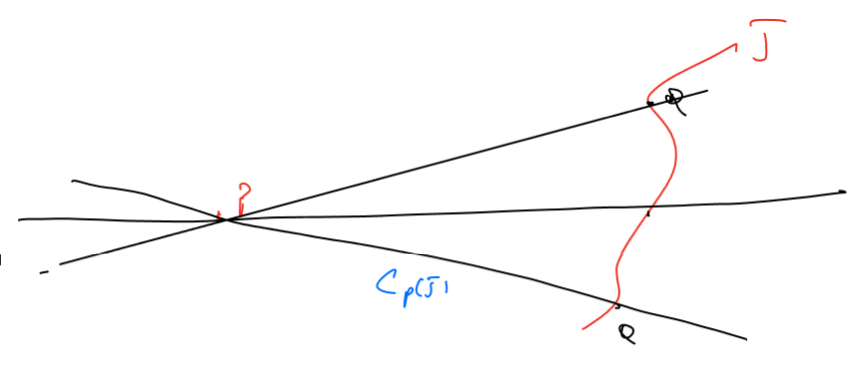
\includegraphics[scale=.53]{cono_proiettivo.png}\\
\end{center}
\textbf{Esercizio}\\
1. $S\subseteq\pro$ è un sottospazio proiettivo, allora 
\[
 C_p(S) = L(P,S) 
.\] 
2. $S_1, S_2$ sono sottospazi proiettivi, allora 
\[
	L(S_1,S_2) = \bigcup_{P_1\in S_1, P_2\in S_2} L(P_1,P_2) = \bigcup_{P_2\in S_2} C_{P_2}(S_1)
.\] 
\ \\ \hline \ \\
$H\in \pro$ iperpiano $P\in \pro\setminus H$\\
La proiezione di  $H$ di centro $P$ è l'applicazione
\[
	\pi_{P,H}:\pro\setminus\{P\} \rightarrow H
.\] 
\[
	\pi_{P,H}(Q) = L(P,Q) \cap H
.\] 
Osserviamo che se $J\subseteq \pro$ e $p\notin J$
 \[
	 \pi_{P,H}(J) = H\cap C_P(J)
.\] 
\textbf{Esempio}\\
$\pro^N, \ \ \ H_0 = \{x_0=0\} = \{[0,x_1,\ldots,x_N]\in \pro^N\}$\\
Dato che punti proporzionali ci danno lo stesso risultato dire $x_0 = 1$ non avrebbe senso, sarebbe identico a $x_0=3$\\[10px]
Se $P = [1,0,\ldots,0]\notin H_0$\\
Se $Q = [x_0,\ldots,x_N]$, allora
\[
	\pi_{P,H}(Q) = [0,x_1,\ldots,x_N]
.\] 
$L(P,Q) = [ \lambda + \mu x_0, \mu x_1,\ldots, \mu x_n]\\$
$L(P,Q)\cap H_0$\\
\textbf{Esempio}\\
$[1,2,1] [0,1,-1]$\\
\[
	\{ \lambda [1,2,1] + \mu [0,1,-1] | ( \lambda,\mu)\in \K^2 \neq(0,0)\}
.\] 
Qui c'è lo spazio quoziente $( \lambda,\mu) / \lambda \sim \mu $
\ \\ \hline \ \\ 
\section{Posizione generale di sottospazi in $\pro^3, \pro^4}$}
 \begin{aligned}
	&\dim S_1 = h\\
	&\dim S_2 = k\\
	&\dim \pro = n 
 \end{aligned}\ \ \ $\dim S_1\cap S_2$ = \begin{cases}
	&h + k - n \ \ \ h + k\geq n\\
	&-1 \ \ \  \ \ \ \ \ \ \ \ h + k < n\\
 \end{cases}\\
 \begin{center}
 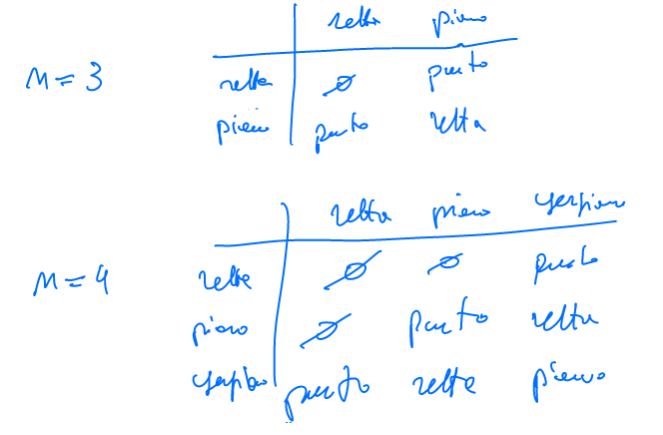
\includegraphics[scale=.5]{tabelle.png}\\
 \end{center}
 \ \\ \hline \ \\
 Osserviamo che in un riferimento proiettivo in $\pro^n$ sia  $e_0,\ldots,e_n$ individua i punti fondamentali ed il punto unità, e questi sono in posizione generale
 \[
	 F_0 = [e_0], \ldots, F_n=[e_n], u  = [e_0 + \ldots + e_n]
 .\] 
 ogni $(n+1)$-ple di righe ha rango massimo
 \begin{aligned}
	& 1 \ \ 0 \ldots \ \ 0\\
	&\dots \ \ \ldots\\
	&0\ \  0 \ldots \ \ 1\\
	&1 \ \ 1\ldots \ \ 1
 \end{aligned}\\
 \textbf{Esempio} $\pro^2$ $[e_0]\ \ \ \ $ \begin{aligned}
	&1 \ 0 \ 0 \\
	&0\ 1 \ 0 \\
	& 0 \ 0 \ 1\\
	&1 \ 1 \ 1
 \end{aligned} $\ \ \ $
 tutti i minori di rango 3 sono non zero\\
 Viceversa, data una $(n+2)$-pla di punti in posizione generale, esiste un unico riferimento proiettivo che il ammette come punti fondamentali e punti unità.\\
 Siano dati $P_0,\ldots,P_n$ n punti in posizione generale, \\supponiamo che $P_i= [v_i] , \ \ i= 0,\ldots,n$\\
 Allora $\{v_0,\ldots,v_n\}$ è una base di $V$. Se $n\in V$ è tale che  $N = [n]$, allora
  \[
 n = \lambda_0v_0+\ldots+ \lambda_n v_n
 .\] 
 in modo unico. \\Osserviamo che per l'ipotesi di posizione generale, tutti i $ \lambda_i$ sono diversi da zero.\\
 Allora $( \lambda_0v_0)\ldots ( \lambda v_n)$ è un riferimento con le proprietà valide: infatti i punti fondamentali sono 
 \[
	 [ \lambda_i v_i] = [v_i] = P_i
 .\] 
 \[
	 [( \lambda_0 v_0) + \ldots +( \lambda_n v_n)] = [n] = V
 .\] 
 \newpage
 \subsection{Esercizi}
 Verificare che in $\pro^2(\R)$
  \[
	  [\frac{1}{2},1,1],\ \ [1,\frac 4 3, \frac 4 3],\ \ [2,-1,2]
 .\] 
 Sono allineati e trovare un'equazione della retta che li contiene\\
 \textbf{Svolgimento}\\[10px]
\begin{agliend}
	0=\det\matrice{x_0&x_1&x_2\\1&2&2\\3&1&4} = 6 x_0 + 2 x_1 - 5x_2 = 12 -2 -10 = 0
\end{agliend}\\
\textbf{Altro Esercizio:}\\
Determinare i valori di $a\in \C$ per cui le rette in  $\pro^2(\C)$
 \[
ax_1 - x_2 + 3ix_0 =0
.\] 
\[
-iax_1 + x_1 - ix_2 = 0
.\] 
\[
3ix_2 + 3x_0 + x_1 = 0
.\] 
sono concorrenti (si intersecano in un punto)\\
\textbf{Svolgimento}\\
Le rette sono concorrenti se e solo se il sistema delle tre equazioni ha una soluzione non nulla
\[
	A = \matrice{3i&a&-1\\-ia&1&-i\\5&1&3i}
.\] 
$\displaystyle\det A  = 0\ \ \ \ ra^2 + 4ia + 7 = 0 \ \ \Rightarrow  \ \ a = \frac{-2 \pm \sqrt{-ra^2-21a^2}}{3} = $ \begin{cases}
	i\\
	-\frac{7}{3}i
\end{cases}\\
\textbf{Altro altro esercizio}\\
Si considerano i punti seguenti in $\pro^3(R)$
 \[
	 P_1 = [1,0,1,2], \ P_2 = [0,1,1,1], \ P_3 = [2,1,2,2], \ P_4=[1,1,2,3]
.\] 
a. Dire se $P_1,P_2,P_3,P_4$ sono in posizione generale\\
b. Calcola $\dim L(P_1,P_2,P_3,P_4$ e trovare equazioni cartesiane\\
c. Completare, se possibile, $P_1,P_2,P_3$ a un riferimento proiettivo di $\pro^3(\R)$\\
 \textbf{Svolgimento}\\
 I punti dati sono in posizione generale se posto $P_i = [v_i]$,  $v_1,v_2,v_3,v_4$ sono linearmente indipendenti
 \[
	 \det\matrice{1&0&1&2\\0&1&1&1\\2&1&2&2\\1&1&2&3}=0
 .\] 
	 Tuttavia il determinante del minore $\matrice{1&0&1\\0&1&1\\0&1&2}$ è diverso da 0 
	  \[
	 L(P_1,P_2,P_3,P_4) = L(P_1,P_2,P_3)
	 .\] 
	 \[
		 \det\matrice{x_0&x_1&x_2&x_3\\1&0&1&2\\0&1&1&1\\2&1&2&2} = 0 \ \ \ \Rightarrow  \ \ -x_0 -2x_1+3x_2-x_3=0
	 .\] 
	 Ultimo punto dell'esercizio\\
	 Per prima cosa si completa ad una base, si può completare con $\icol{0\\0\\0\\1}$ e il determinate è diverso da 0, a questo punto possiamo prendere  $P_1,P_2,P_3$ come prima, $\widetilde{P}^4 = [0,0,0,1] $  $ U = [3,2,4,6]$

\end{document}

